% Options for packages loaded elsewhere
% Options for packages loaded elsewhere
\PassOptionsToPackage{unicode}{hyperref}
\PassOptionsToPackage{hyphens}{url}
\PassOptionsToPackage{dvipsnames,svgnames,x11names}{xcolor}
%
\documentclass[
  11pt,
]{article}
\usepackage{xcolor}
\usepackage[margin=0.5in]{geometry}
\usepackage{amsmath,amssymb}
\setcounter{secnumdepth}{-\maxdimen} % remove section numbering
\usepackage{iftex}
\ifPDFTeX
  \usepackage[T1]{fontenc}
  \usepackage[utf8]{inputenc}
  \usepackage{textcomp} % provide euro and other symbols
\else % if luatex or xetex
  \usepackage{unicode-math} % this also loads fontspec
  \defaultfontfeatures{Scale=MatchLowercase}
  \defaultfontfeatures[\rmfamily]{Ligatures=TeX,Scale=1}
\fi
\usepackage{lmodern}
\ifPDFTeX\else
  % xetex/luatex font selection
\fi
% Use upquote if available, for straight quotes in verbatim environments
\IfFileExists{upquote.sty}{\usepackage{upquote}}{}
\IfFileExists{microtype.sty}{% use microtype if available
  \usepackage[]{microtype}
  \UseMicrotypeSet[protrusion]{basicmath} % disable protrusion for tt fonts
}{}
\makeatletter
\@ifundefined{KOMAClassName}{% if non-KOMA class
  \IfFileExists{parskip.sty}{%
    \usepackage{parskip}
  }{% else
    \setlength{\parindent}{0pt}
    \setlength{\parskip}{6pt plus 2pt minus 1pt}}
}{% if KOMA class
  \KOMAoptions{parskip=half}}
\makeatother
% Make \paragraph and \subparagraph free-standing
\makeatletter
\ifx\paragraph\undefined\else
  \let\oldparagraph\paragraph
  \renewcommand{\paragraph}{
    \@ifstar
      \xxxParagraphStar
      \xxxParagraphNoStar
  }
  \newcommand{\xxxParagraphStar}[1]{\oldparagraph*{#1}\mbox{}}
  \newcommand{\xxxParagraphNoStar}[1]{\oldparagraph{#1}\mbox{}}
\fi
\ifx\subparagraph\undefined\else
  \let\oldsubparagraph\subparagraph
  \renewcommand{\subparagraph}{
    \@ifstar
      \xxxSubParagraphStar
      \xxxSubParagraphNoStar
  }
  \newcommand{\xxxSubParagraphStar}[1]{\oldsubparagraph*{#1}\mbox{}}
  \newcommand{\xxxSubParagraphNoStar}[1]{\oldsubparagraph{#1}\mbox{}}
\fi
\makeatother


\usepackage{longtable,booktabs,array}
\usepackage{calc} % for calculating minipage widths
% Correct order of tables after \paragraph or \subparagraph
\usepackage{etoolbox}
\makeatletter
\patchcmd\longtable{\par}{\if@noskipsec\mbox{}\fi\par}{}{}
\makeatother
% Allow footnotes in longtable head/foot
\IfFileExists{footnotehyper.sty}{\usepackage{footnotehyper}}{\usepackage{footnote}}
\makesavenoteenv{longtable}
\usepackage{graphicx}
\makeatletter
\newsavebox\pandoc@box
\newcommand*\pandocbounded[1]{% scales image to fit in text height/width
  \sbox\pandoc@box{#1}%
  \Gscale@div\@tempa{\textheight}{\dimexpr\ht\pandoc@box+\dp\pandoc@box\relax}%
  \Gscale@div\@tempb{\linewidth}{\wd\pandoc@box}%
  \ifdim\@tempb\p@<\@tempa\p@\let\@tempa\@tempb\fi% select the smaller of both
  \ifdim\@tempa\p@<\p@\scalebox{\@tempa}{\usebox\pandoc@box}%
  \else\usebox{\pandoc@box}%
  \fi%
}
% Set default figure placement to htbp
\def\fps@figure{htbp}
\makeatother





\setlength{\emergencystretch}{3em} % prevent overfull lines

\providecommand{\tightlist}{%
  \setlength{\itemsep}{0pt}\setlength{\parskip}{0pt}}



 


\usepackage{fancyhdr}
\usepackage{graphicx}
\usepackage{xcolor}
\usepackage{booktabs}
\usepackage{multicol}
\usepackage{float}
\definecolor{primary}{RGB}{25,25,112}
\definecolor{secondary}{RGB}{178,34,34}
\definecolor{mapred}{RGB}{255,0,0}
\definecolor{maporange}{RGB}{255,165,0}
\definecolor{mapgreen}{RGB}{0,128,0}
\definecolor{mapblue}{RGB}{0,0,255}
\definecolor{mappurple}{RGB}{128,0,128}
\definecolor{brown}{RGB}{139,69,19}
\definecolor{gold}{RGB}{255,215,0}
\definecolor{cyan}{RGB}{0,255,255}
\definecolor{gray}{RGB}{128,128,128}
\definecolor{darkblue}{RGB}{0,0,139}
\definecolor{darkred}{RGB}{139,0,0}
\definecolor{purple}{RGB}{128,0,128}
\pagestyle{fancy}
\fancyhf{}
\fancyhead[L]{\textcolor{primary}{\textbf{Smadar's Booking Guide}}}
\fancyhead[R]{\textcolor{secondary}{\textbf{PNW Adventure 2025}}}
\fancyfoot[C]{\thepage}
\renewcommand{\headrulewidth}{0.4pt}
\makeatletter
\@ifpackageloaded{caption}{}{\usepackage{caption}}
\AtBeginDocument{%
\ifdefined\contentsname
  \renewcommand*\contentsname{Table of contents}
\else
  \newcommand\contentsname{Table of contents}
\fi
\ifdefined\listfigurename
  \renewcommand*\listfigurename{List of Figures}
\else
  \newcommand\listfigurename{List of Figures}
\fi
\ifdefined\listtablename
  \renewcommand*\listtablename{List of Tables}
\else
  \newcommand\listtablename{List of Tables}
\fi
\ifdefined\figurename
  \renewcommand*\figurename{Figure}
\else
  \newcommand\figurename{Figure}
\fi
\ifdefined\tablename
  \renewcommand*\tablename{Table}
\else
  \newcommand\tablename{Table}
\fi
}
\@ifpackageloaded{float}{}{\usepackage{float}}
\floatstyle{ruled}
\@ifundefined{c@chapter}{\newfloat{codelisting}{h}{lop}}{\newfloat{codelisting}{h}{lop}[chapter]}
\floatname{codelisting}{Listing}
\newcommand*\listoflistings{\listof{codelisting}{List of Listings}}
\makeatother
\makeatletter
\makeatother
\makeatletter
\@ifpackageloaded{caption}{}{\usepackage{caption}}
\@ifpackageloaded{subcaption}{}{\usepackage{subcaption}}
\makeatother
\usepackage{bookmark}
\IfFileExists{xurl.sty}{\usepackage{xurl}}{} % add URL line breaks if available
\urlstyle{same}
\hypersetup{
  pdftitle={Smadar's Booking Booklet},
  pdfauthor={Complete Booking Guide with Enhanced Geospatial Maps},
  colorlinks=true,
  linkcolor={blue},
  filecolor={Maroon},
  citecolor={Blue},
  urlcolor={Blue},
  pdfcreator={LaTeX via pandoc}}


\title{Smadar's Booking Booklet}
\usepackage{etoolbox}
\makeatletter
\providecommand{\subtitle}[1]{% add subtitle to \maketitle
  \apptocmd{\@title}{\par {\large #1 \par}}{}{}
}
\makeatother
\subtitle{Pacific Northwest Adventure 2025}
\author{Complete Booking Guide with Enhanced Geospatial Maps}
\date{2014-08-03}
\begin{document}
\maketitle


\section{\texorpdfstring{\textcolor{primary}{Trip Overview \& Emergency Contacts}}{}}\label{section}

\textbf{\textcolor{secondary}{Travelers:}} Aviv \& Smadar\\
\textbf{\textcolor{secondary}{Duration:}} August 3-12, 2025 (departing
Seattle Aug 12)\\
\textbf{\textcolor{secondary}{Total Distance:}} 1,049 miles \textbar{}
\textbf{\textcolor{secondary}{Total Driving Time:}} 20.4 hours

\textbf{\textcolor{primary}{Emergency Contact:}} Gil \& Camila
(traveling companions)

\subsection{\texorpdfstring{\textcolor{primary}{UPDATED BOOKING PRIORITIES}}{}}\label{section-1}

✅ \textbf{\textcolor{primary}{COMPLETED:}} Kimpton Bozeman (Aug 3-5) -
Two King Rooms\\
✅ \textbf{\textcolor{primary}{COMPLETED:}} Under Canvas Columbia River
Gorge (Aug 11) - Stargazers Tent

\textbf{\textcolor{secondary}{REMAINING URGENT PRIORITIES:}}

\begin{enumerate}
\def\labelenumi{\arabic{enumi}.}
\item
  \textbf{\textcolor{primary}{FLIGHTS}} - August 3rd to Bozeman
  (\textasciitilde\$109/person vs \$349 Aug 4th)
\item
  \textbf{\textcolor{primary}{LA CASA ITALIANA McCall}} - Book the condo
  for Aug 6-8
\item
  \textbf{\textcolor{primary}{The Jennings Hotel Joseph}} - Little Brick
  Building + Room \#11 for Aug 8-9
\end{enumerate}

\begin{center}\rule{0.5\linewidth}{0.5pt}\end{center}

\newpage

\section{\texorpdfstring{\textcolor{primary}{LEG 1: Bozeman, Montana}}{}}\label{section-2}

\subsection{\texorpdfstring{\textcolor{secondary}{August 3-4, 2025 | 2 Nights}}{}}\label{section-3}

\textbf{\textcolor{secondary}{Arrival Route:}} Flight to
Bozeman-Yellowstone International (BZN)

\subsubsection{\texorpdfstring{\textcolor{primary}{BOOKING STATUS: ✅ BOOKED!}}{}}\label{section-4}

\textbf{\textcolor{secondary}{Hotel:}} Kimpton Armory Hotel Bozeman\\
\textbf{\textcolor{secondary}{Address:}} 24 W Mendenhall St, Bozeman, MT
59715\\
\textbf{\textcolor{secondary}{Phone:}} (406) 551-7700 \textbar{}
\textbf{\textcolor{secondary}{Website:}} kimptonarmoryhotel.com\\
\textbf{\textcolor{primary}{CONFIRMED:}} Two King Rooms for August 3-5,
2025\\
\textbf{\textcolor{primary}{Status:}} ✅ SUCCESSFULLY BOOKED BY SMADAR

\subsubsection{\texorpdfstring{\textcolor{primary}{ROUTE INFORMATION}}{}}\label{section-5}

\textbf{\textcolor{secondary}{Arrival:}} Fly into Bozeman-Yellowstone
International (BZN)\\
\textbf{\textcolor{secondary}{Departure:}} Drive to Missoula (202 mi, 2h
58m)

\subsubsection{\texorpdfstring{\textcolor{primary}{FLIGHT BOOKING (STILL NEEDED)}}{}}\label{section-6}

\textbf{\textcolor{secondary}{To Bozeman (August 3rd):}}\\
- \textbf{RECOMMENDED:} Morning flight JFK→BZN\\
- \textbf{Cost:} \$109/person (SAVE \$240 vs Aug 4th)\\
- \textbf{Flight Time:} 5h 5m direct Delta\\
- \textbf{\textcolor{secondary}{URGENT:}} Book immediately for savings

\subsubsection{\texorpdfstring{\textcolor{primary}{DINING RESERVATIONS NEEDED}}{}}\label{section-7}

\begin{itemize}
\tightlist
\item
  \textbf{\textcolor{secondary}{Blackbird Kitchen}} - Wood-fired
  Argentine lamb (dinner reservation recommended)
\item
  \textbf{\textcolor{secondary}{Montana Ale Works}} - Local brewery in
  historic railroad building
\item
  \textbf{\textcolor{secondary}{Wild Crumb Bakery}} - European-style
  breakfast breads
\end{itemize}

\subsubsection{\texorpdfstring{\textcolor{primary}{ACTIVITIES TO BOOK}}{}}\label{section-8}

\begin{itemize}
\tightlist
\item
  \textbf{\textcolor{secondary}{Museum of the Rockies}} - Dinosaur
  exhibits (no reservation needed)
\item
  \textbf{\textcolor{secondary}{Montana State University Campus}} -
  Self-guided tour available
\item
  \textbf{\textcolor{secondary}{Downtown Bozeman Walking Tour}} - Check
  with hotel concierge
\end{itemize}

\newpage

\section{\texorpdfstring{\textcolor{primary}{LEG 1: Bozeman Enhanced Geospatial Context}}{}}\label{section-9}

\begin{figure}[H]
\centering

\includegraphics[width=0.9\textwidth]{images/bozeman_mt_geomorphological_map.png}
\caption{\textbf{\textcolor{primary}{BOZEMAN \& GALLATIN VALLEY • Enhanced Geomorphological Context}} \\ 
\textbf{\textcolor{secondary}{Accommodation:}} \textcolor{mapred}{●} Kimpton Armory Hotel (Red Star) \\
\textbf{\textcolor{secondary}{Geological Features:}} \\
\textcolor{brown}{●} \textcolor{brown}{Gallatin Valley} (intermontane basin) \\
\textcolor{gray}{●} \textcolor{gray}{Glacial Lake Missoula Influence} (Ice Age flood impacts) \\
\textcolor{mapgreen}{●} \textcolor{mapgreen}{Gallatin River} (Rocky Mountain drainage) \\
\textcolor{mapblue}{●} \textcolor{mapblue}{Bridger Mountains} (northern boundary) \\
\textbf{\textcolor{secondary}{Key Locations:}} \\
\textcolor{mapred}{★} Downtown Historic District • Montana State University • Museum of the Rockies}
\end{figure}

\begin{center}\rule{0.5\linewidth}{0.5pt}\end{center}

\newpage

\section{\texorpdfstring{\textcolor{primary}{LEG 2: Missoula, Montana}}{}}\label{section-10}

\subsection{\texorpdfstring{\textcolor{secondary}{August 5, 2025 | 1 Night}}{}}\label{section-11}

\textbf{\textcolor{secondary}{Driving Route:}} Bozeman → Missoula (202
mi, 2h 58m)

\subsubsection{\texorpdfstring{\textcolor{primary}{BOOKING DETAILS}}{}}\label{section-12}

\textbf{\textcolor{secondary}{Hotel:}} AC Hotel Missoula Downtown\\
\textbf{\textcolor{secondary}{Address:}} 200 S Pattee St, Missoula, MT
59802\\
\textbf{\textcolor{secondary}{Phone:}} (406) 541-8000\\
\textbf{\textcolor{secondary}{Website:}}
marriott.com/en-us/hotels/msoac-ac-hotel-missoula-downtown\\
\textbf{\textcolor{secondary}{Rate:}} \$455/night per room (need 2
rooms) \textbar{} \textbf{\textcolor{secondary}{Total:}} \$910\\
\textbf{\textcolor{secondary}{Room Request:}} ``High floor, west-facing
corner room with panoramic city views''

\subsubsection{\texorpdfstring{\textcolor{primary}{ROUTE INFORMATION}}{}}\label{section-13}

\textbf{\textcolor{secondary}{From:}} Bozeman, MT \textbar{}
\textbf{\textcolor{secondary}{Distance:}} 202 miles \textbar{}
\textbf{\textcolor{secondary}{Drive Time:}} 2h 58m\\
\textbf{\textcolor{secondary}{Next Day:}} Drive to Jerry Johnson Hot
Springs (66 mi, 1h 20m)

\subsubsection{\texorpdfstring{\textcolor{primary}{DINING RESERVATIONS NEEDED}}{}}\label{section-14}

\begin{itemize}
\tightlist
\item
  \textbf{\textcolor{secondary}{Le Petit Outre}} - French bistro (dinner
  reservation recommended)
\item
  \textbf{\textcolor{secondary}{Plonk Wine Bar}} - Montana wine
  selection
\item
  \textbf{\textcolor{secondary}{Ask hotel concierge}} for local brewery
  recommendations
\end{itemize}

\subsubsection{\texorpdfstring{\textcolor{primary}{ACTIVITIES}}{}}\label{section-15}

\begin{itemize}
\tightlist
\item
  \textbf{\textcolor{secondary}{Clark Fork Riverfront Trail}} -
  Riverside walking path
\item
  \textbf{\textcolor{secondary}{University of Montana}} - Historic
  campus exploration
\item
  \textbf{\textcolor{secondary}{Rocky Mountain Elk Foundation}} -
  Wildlife education center
\end{itemize}

\newpage

\section{\texorpdfstring{\textcolor{primary}{LEG 2: Missoula Enhanced Geospatial Context}}{}}\label{section-16}

\begin{figure}[H]
\centering
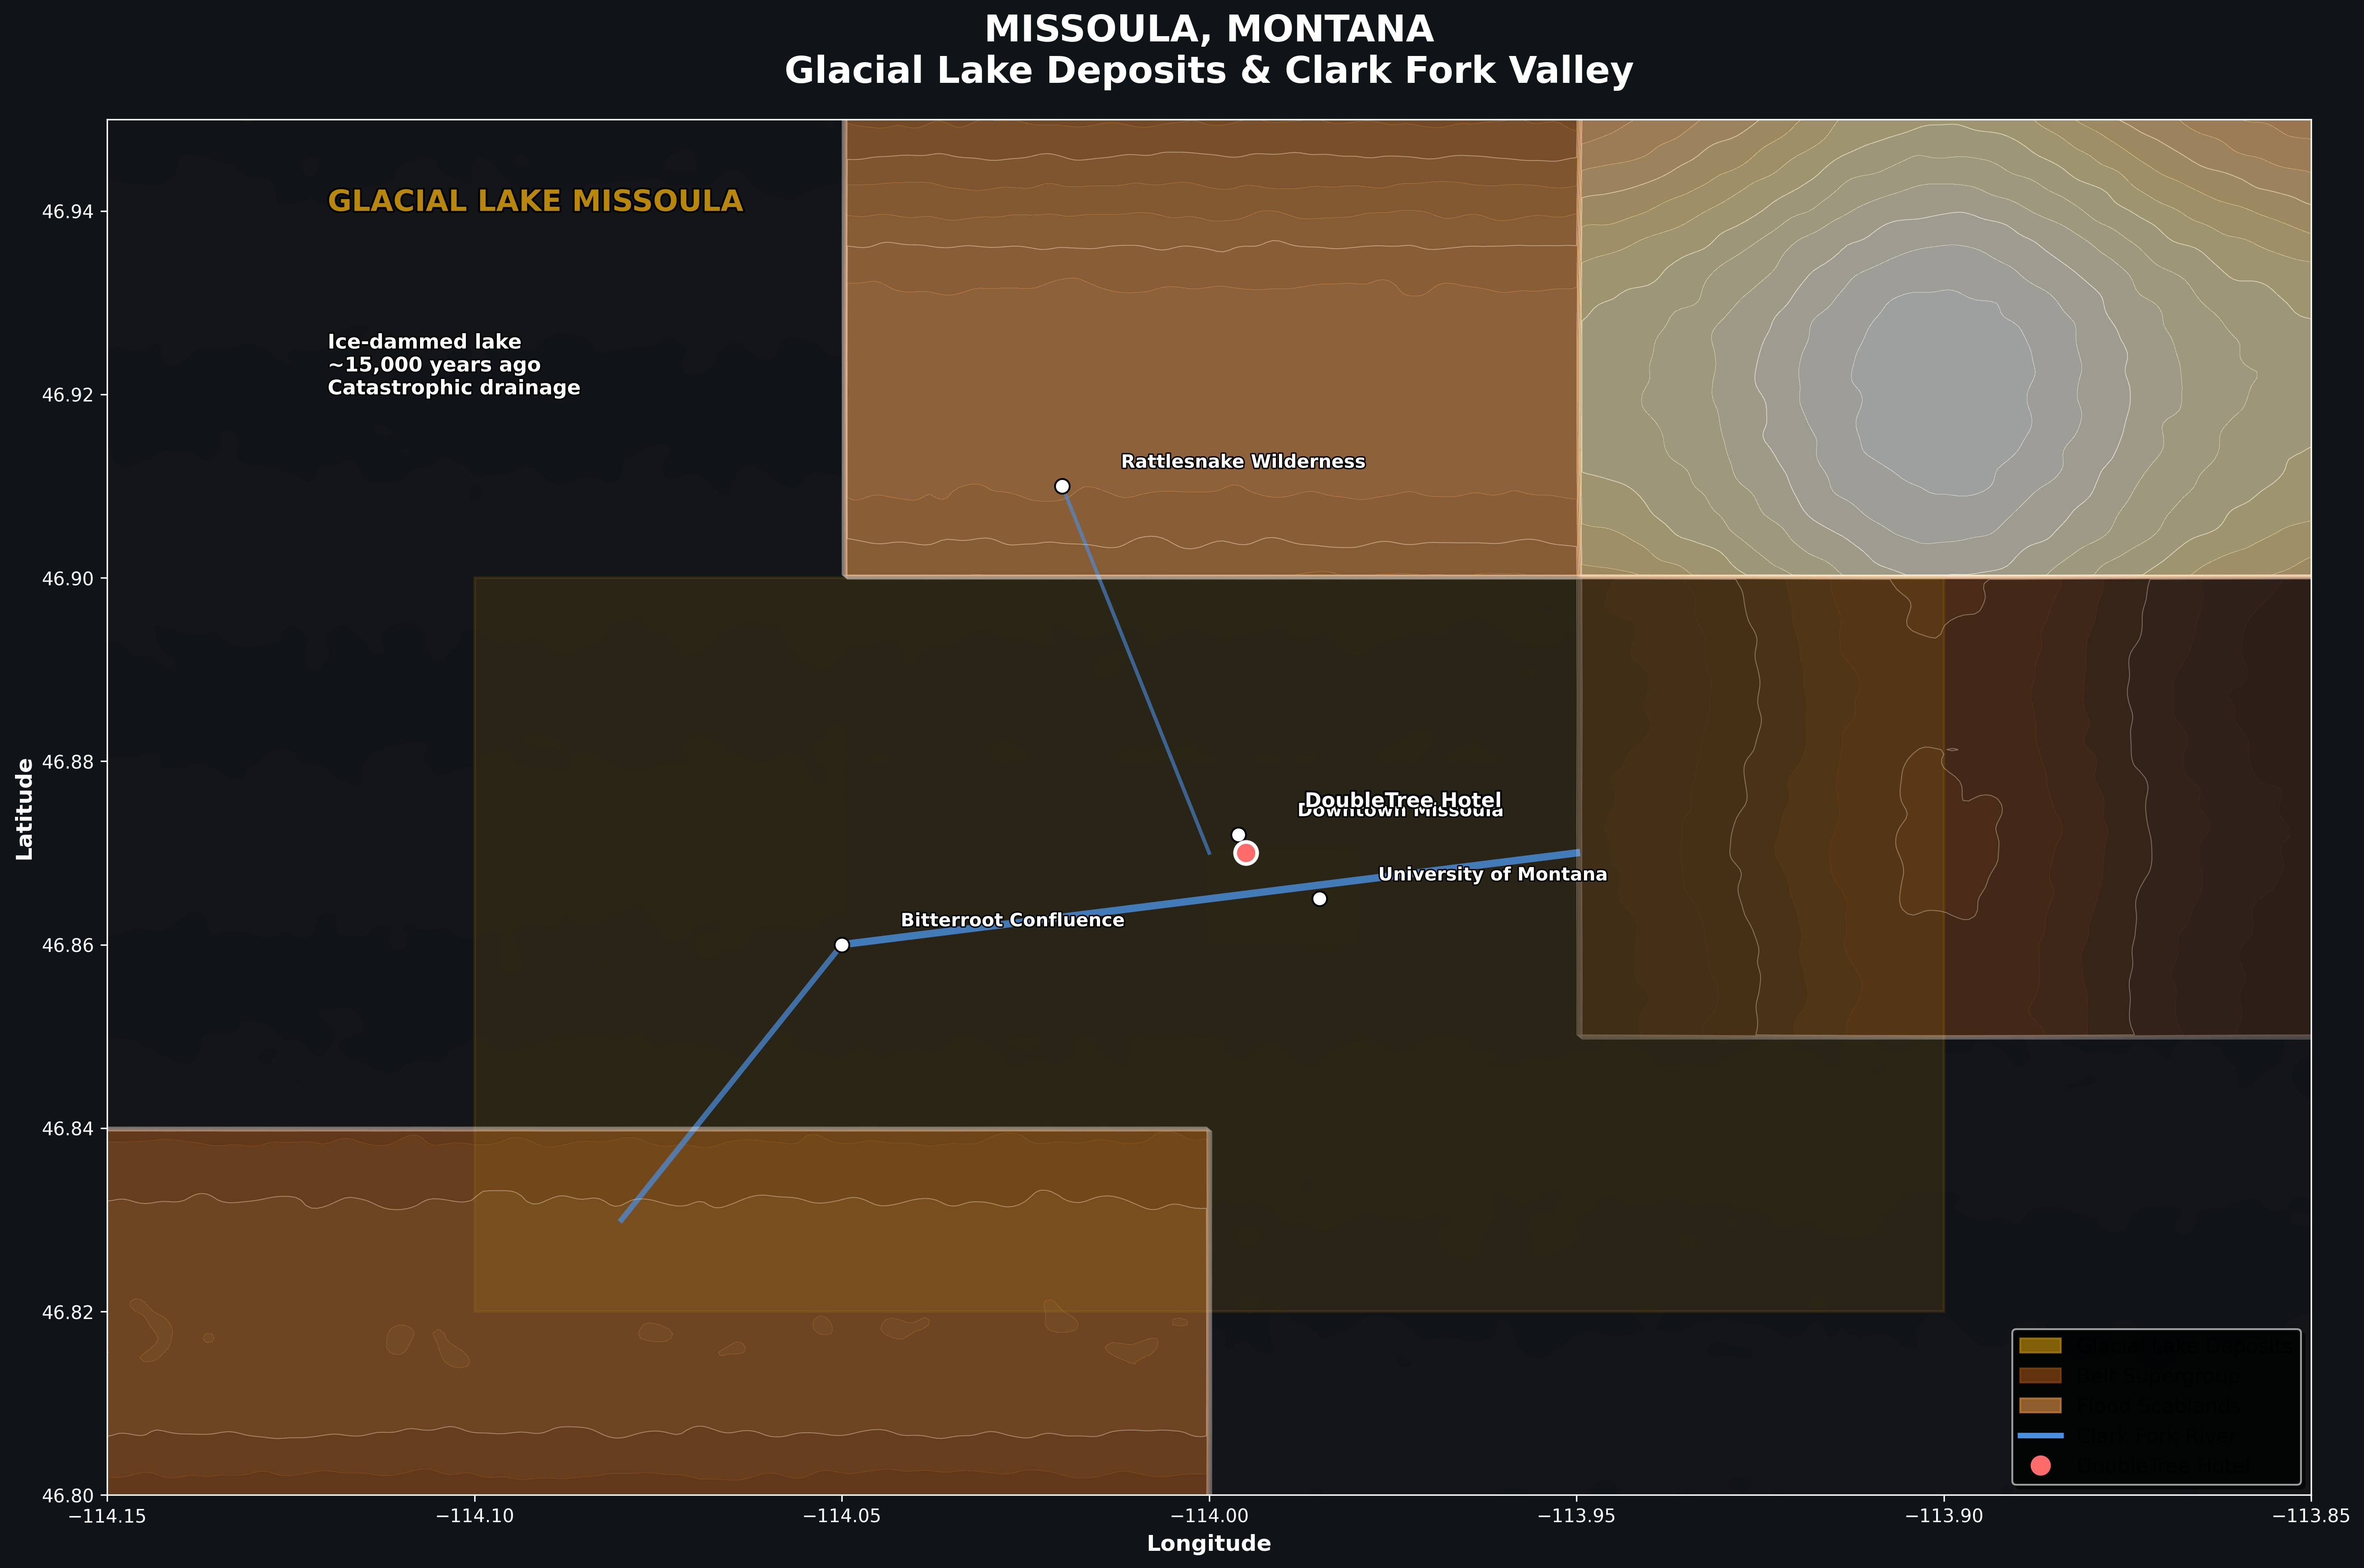
\includegraphics[width=0.9\textwidth]{images/missoula_enhanced_geospatial.png}
\caption{\textbf{\textcolor{primary}{MISSOULA \& GLACIAL LAKE MISSOULA • Enhanced Geomorphological Context}} \\ 
\textbf{\textcolor{secondary}{Accommodation:}} \textcolor{mapred}{●} AC Hotel Missoula Downtown (Red Star) \\
\textbf{\textcolor{secondary}{Geological Features:}} \\
\textcolor{mapblue}{●} \textcolor{mapblue}{Clark Fork River} (glacial outburst flood channel) \\
\textcolor{brown}{●} \textcolor{brown}{Glacial Lake Missoula Deposits} (rhythmite layers) \\
\textcolor{gray}{●} \textcolor{gray}{Missoula Flood Gravels} (Ice Age megaflood deposits) \\
\textcolor{mapgreen}{●} \textcolor{mapgreen}{Glacial Lake Terraces} (former shoreline benches) \\
\textbf{\textcolor{secondary}{Key Locations:}} \\
\textcolor{mapred}{★} Downtown Missoula • University of Montana • Riverfront Trail • Mount Sentinel}
\end{figure}

\begin{center}\rule{0.5\linewidth}{0.5pt}\end{center}

\newpage

\section{\texorpdfstring{\textcolor{primary}{LEG 3: McCall, Idaho}}{}}\label{section-17}

\subsection{\texorpdfstring{\textcolor{secondary}{August 6-8, 2025 | 2 Nights}}{}}\label{section-18}

\textbf{\textcolor{secondary}{Driving Route:}} Missoula → Jerry Johnson
→ McCall (256 mi total, 5h 9m with hot springs stop)

\subsubsection{\texorpdfstring{\textcolor{primary}{BOOKING DETAILS}}{}}\label{section-19}

\textbf{\textcolor{secondary}{Property:}} LA CASA ITALIANA - Charming
Tri-Level Condo\\
\textbf{\textcolor{secondary}{Location:}} Downtown McCall, ID\\
\textbf{\textcolor{secondary}{Rate:}} \$360/night -
\textbf{\textcolor{primary}{TOTAL \$1,080}} for 3 nights (Aug 6-8)\\
\textbf{\textcolor{secondary}{Type:}} Condominium - 6 guests, 3
bedrooms, 2 bathrooms\\
\textbf{\textcolor{secondary}{Booking:}} Vacation rental platforms -
Search ``La Casa Italiana McCall''

\subsubsection{\texorpdfstring{\textcolor{primary}{ROUTE INFORMATION}}{}}\label{section-20}

\textbf{\textcolor{secondary}{August 6:}} Missoula → Jerry Johnson Hot
Springs (66 mi, 1h 20m)\\
\textbf{\textcolor{secondary}{Stop:}} Jerry Johnson Hot Springs (day
visit - FREE, 6 AM-8 PM)\\
\textbf{\textcolor{secondary}{Continue:}} Jerry Johnson → McCall (190
mi, 3h 49m)

\subsubsection{\texorpdfstring{\textcolor{primary}{CONDO ADVANTAGES}}{}}\label{section-21}

\begin{itemize}
\tightlist
\item
  \textbf{\textcolor{secondary}{Full kitchen}} for meal preparation
  \textbar{} \textbf{\textcolor{secondary}{Fireplace}} for cozy
  evenings\\
\item
  \textbf{\textcolor{secondary}{Downtown location}} - walk to shops,
  restaurants, Payette Lake\\
\item
  \textbf{\textcolor{secondary}{Much more space}} than hotel rooms
  \textbar{} \textbf{\textcolor{secondary}{Cost savings}} vs Shore Lodge
\end{itemize}

\subsubsection{\texorpdfstring{\textcolor{primary}{HOT SPRINGS DAY TRIPS}}{}}\label{section-22}

\begin{itemize}
\tightlist
\item
  \textbf{\textcolor{secondary}{Jerry Johnson Hot Springs}} - Rock
  pools, 60-foot walk from parking
\item
  \textbf{\textcolor{secondary}{Burgdorf Hot Springs}} - Historic resort
  (\$20/adult, reservations required)
\item
  \textbf{\textcolor{secondary}{Gold Fork Hot Springs}} - Six tiered
  pools (\$10/adult)
\end{itemize}

\newpage

\section{\texorpdfstring{\textcolor{primary}{LEG 3: McCall Enhanced Geospatial Context}}{}}\label{section-23}

\begin{figure}[H]
\centering
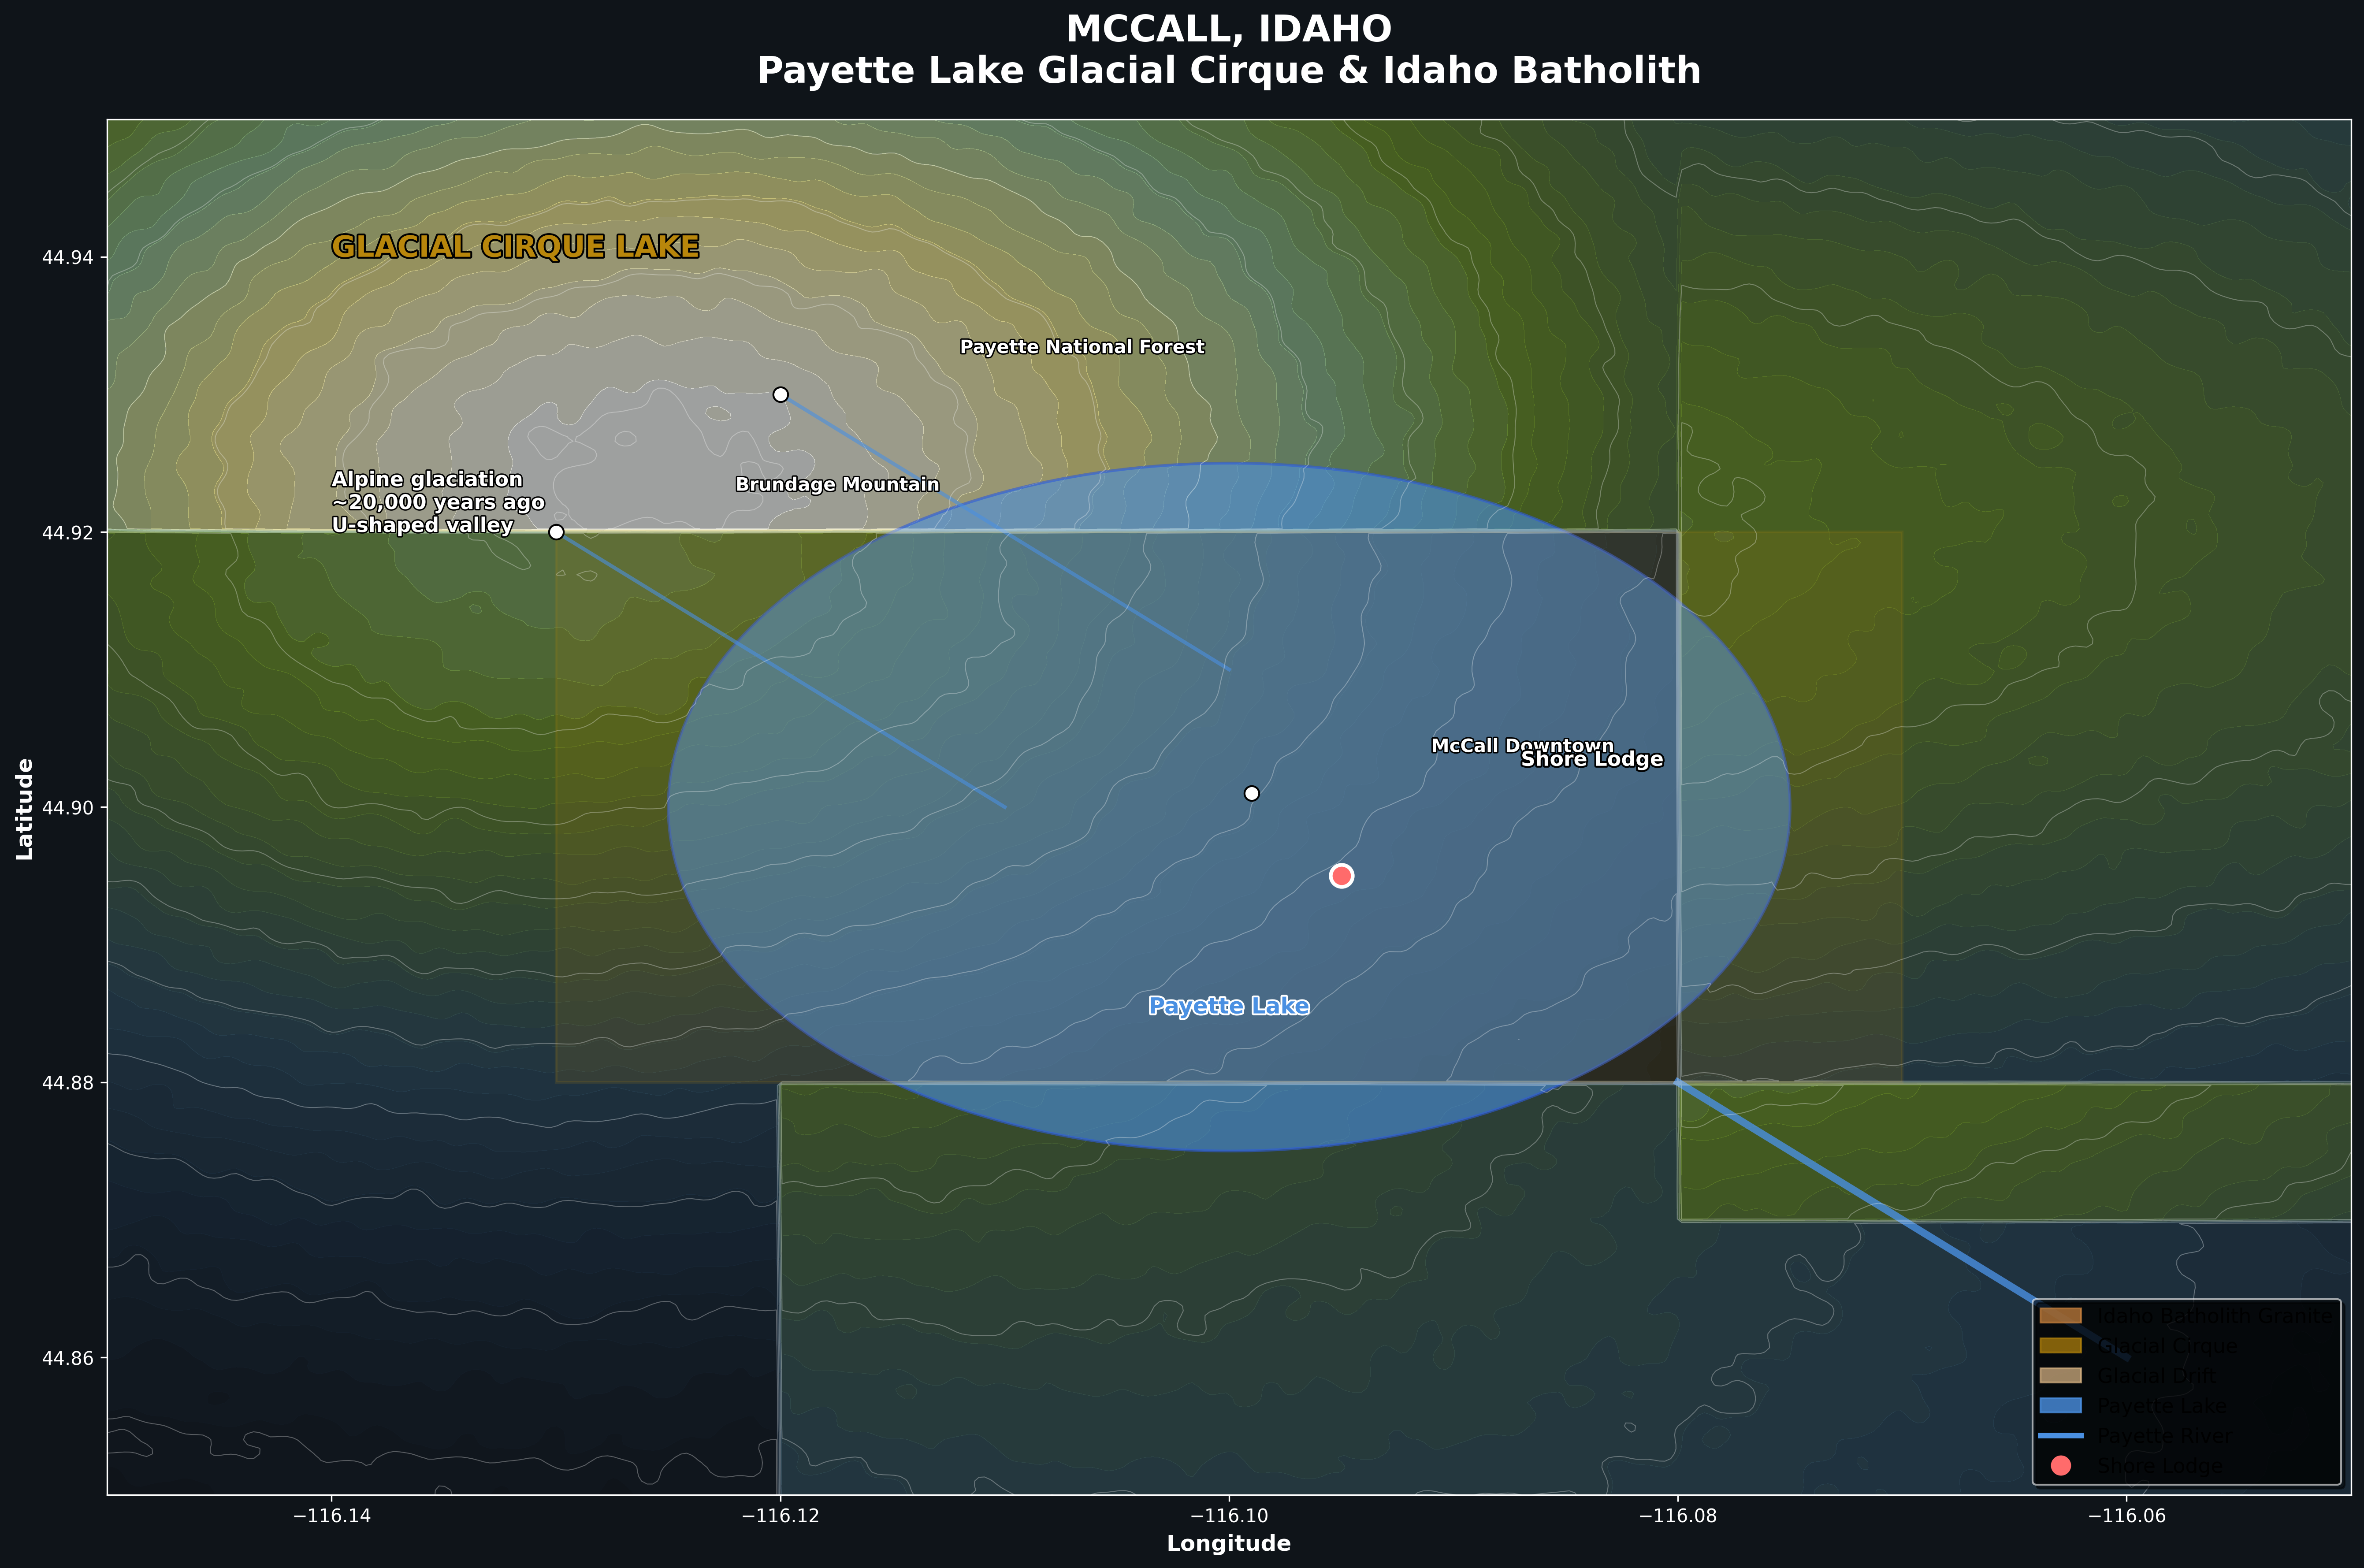
\includegraphics[width=0.9\textwidth]{images/mccall_enhanced_geospatial.png}
\caption{\textbf{\textcolor{primary}{MCCALL \& PAYETTE LAKE • Enhanced Geomorphological Context}} \\ 
\textbf{\textcolor{secondary}{Accommodation:}} \textcolor{mapred}{●} LA CASA ITALIANA Condo (Red Star) \\
\textbf{\textcolor{secondary}{Geological Features:}} \\
\textcolor{brown}{●} \textcolor{brown}{Idaho Batholith} (Cretaceous granite intrusion) \\
\textcolor{mapblue}{●} \textcolor{mapblue}{Payette Lake} (glacial cirque lake) \\
\textcolor{gray}{●} \textcolor{gray}{Glacial Moraines} (Pleistocene ice deposits) \\
\textcolor{mapgreen}{●} \textcolor{mapgreen}{Coniferous Forest} (montane ecosystem) \\
\textbf{\textcolor{secondary}{Key Locations:}} \\
\textcolor{mapred}{★} Downtown McCall • Payette Lake Beach • Legacy Park • Activity Barn}
\end{figure}

\begin{center}\rule{0.5\linewidth}{0.5pt}\end{center}

\newpage

\section{\texorpdfstring{\textcolor{primary}{LEG 4: Joseph, Oregon}}{}}\label{section-24}

\subsection{\texorpdfstring{\textcolor{secondary}{August 8-9, 2025 | 2 Nights}}{}}\label{section-25}

\textbf{\textcolor{secondary}{Driving Route:}} McCall → Joseph (166 mi,
4h 19m through mountain roads)

\subsubsection{\texorpdfstring{\textcolor{primary}{BOOKING DETAILS - TWO ROOMS}}{}}\label{section-26}

\textbf{\textcolor{secondary}{Hotel:}} The Jennings Hotel\\
\textbf{\textcolor{secondary}{Address:}} 100 Main St, Joseph, OR 97846

\textbf{\textcolor{primary}{ROOM 1:}} \textbf{The Little Brick Building}
- \$754 for 2 nights\\
\textbf{\textcolor{secondary}{Features:}} Historic brick cottage with
full kitchen, private bath

\textbf{\textcolor{primary}{ROOM 2:}} \textbf{Room \#11 - Private Bath,
Self Check-in} - \$580 for 2 nights\\
\textbf{\textcolor{secondary}{Features:}} Private bathroom, self
check-in convenience

\textbf{\textcolor{primary}{TOTAL FOR BOTH ROOMS:}} \$1,334 for 2 nights

\subsubsection{\texorpdfstring{\textcolor{primary}{Why This is Premium Despite Rating}}{}}\label{section-27}

\textbf{\textcolor{secondary}{This is a historic, artisanal property}}
like boutique European hotels

\textbf{\textcolor{primary}{Why Star Ratings Are Misleading:}} - Star
ratings favor chain hotels over unique character - Artwork and
furnishings cost thousands - museum-quality pieces\\
- This IS the premium accommodation in the Wallowa Mountains region

\textbf{\textcolor{primary}{Regional Context:}} - Joseph is an arts
destination, not commercial tourism hub - Alternative accommodations are
basic motels in Enterprise (20 minutes away)\\
- This will be the most memorable accommodation of the entire trip

\subsubsection{\texorpdfstring{\textcolor{primary}{ROUTE INFORMATION}}{}}\label{section-28}

\textbf{\textcolor{secondary}{From:}} McCall, ID \textbar{}
\textbf{\textcolor{secondary}{Distance:}} 166 miles \textbar{}
\textbf{\textcolor{secondary}{Drive Time:}} 4h 19m\\
\textbf{\textcolor{secondary}{Stop En Route:}} Lostine, OR (M. Crow \&
Co.~Store)

\subsubsection{\texorpdfstring{\textcolor{primary}{BOOKING LANGUAGE}}{}}\label{section-29}

\emph{``We would like to book TWO rooms for August 8-10, 2025: The
Little Brick Building (\$754) and Room \#11 (\$580). Total booking
\$1,334 for both rooms, 2 nights.''}

\newpage

\section{\texorpdfstring{\textcolor{primary}{LEG 4: Joseph Enhanced Geospatial Context}}{}}\label{section-30}

\begin{figure}[H]
\centering
\includegraphics[width=0.9\textwidth]{images/joseph_enhanced_geospatial.png}
\caption{\textbf{\textcolor{primary}{JOSEPH \& WALLOWA MOUNTAINS • Enhanced Geomorphological Context}} \\ 
\textbf{\textcolor{secondary}{Accommodation:}} \textcolor{mapred}{●} The Jennings Hotel (Red Star) \\
\textbf{\textcolor{secondary}{Geological Features:}} \\
\textcolor{brown}{●} \textcolor{brown}{Wallowa Granite Batholith} (165 Ma "Alps of Oregon") \\
\textcolor{mapblue}{●} \textcolor{mapblue}{Alpine Glacial Cirques} (bowl-shaped amphitheaters) \\
\textcolor{darkblue}{●} \textcolor{darkblue}{Wallowa Lake} (glacial lake, terminal moraine dam) \\
\textcolor{purple}{●} \textcolor{purple}{Hanging Valleys} (tributary valleys left by glaciers) \\
\textcolor{cyan}{●} \textcolor{cyan}{Alpine Waterfalls} (cascades from hanging valleys) \\
\textbf{\textcolor{secondary}{Key Locations:}} \\
\textcolor{mapred}{★} Downtown Joseph • Chief Joseph Mountain • Wallowa Lake • Valley Bronze}
\end{figure}

\subsubsection{\texorpdfstring{\textcolor{primary}{LOSTINE GLACIAL VALLEY ENHANCED GEOSPATIAL CONTEXT}}{}}\label{section-31}

\begin{figure}[H]
\centering
\includegraphics[width=0.9\textwidth]{images/lostine_enhanced_geospatial.png}
\caption{\textbf{\textcolor{primary}{LOSTINE GLACIAL VALLEY • Enhanced Geomorphological Context}} \\ 
\textbf{\textcolor{secondary}{Key Location:}} \textcolor{mapred}{●} M. Crow \& Co. General Store (Red Star) \\
\textbf{\textcolor{secondary}{Geological Features:}} \\
\textcolor{brown}{●} \textcolor{brown}{Wallowa Granite Batholith} (165 Ma Jurassic granite intrusion) \\
\textcolor{mapblue}{●} \textcolor{mapblue}{U-Shaped Glacial Valley} (Pleistocene ice carving) \\
\textcolor{cyan}{●} \textcolor{cyan}{Lostine River} (alpine drainage system) \\
\textcolor{gray}{●} \textcolor{gray}{Glacial Moraines} (terminal and lateral deposits) \\
\textbf{\textcolor{secondary}{Key Features:}} \\
\textcolor{mapred}{★} Historic Mountain Town • Granite Outcrops • Valley Floor Terraces}
\end{figure}

\begin{center}\rule{0.5\linewidth}{0.5pt}\end{center}

\newpage

\section{\texorpdfstring{\textcolor{primary}{LEG 5: Walla Walla, Washington}}{}}\label{section-32}

\subsection{\texorpdfstring{\textcolor{secondary}{August 10, 2025 | 1 Night}}{}}\label{section-33}

\textbf{\textcolor{secondary}{Driving Route:}} Joseph → Walla Walla (109
mi, 2h 11m to wine country)

\subsubsection{\texorpdfstring{\textcolor{primary}{BOOKING DETAILS}}{}}\label{section-34}

\textbf{\textcolor{secondary}{Resort:}} Eritage Resort\\
\textbf{\textcolor{secondary}{Address:}} 1000 N 2nd Ave, Walla Walla, WA
99362\\
\textbf{\textcolor{secondary}{Phone:}} Search needed - try (509)
394-4700\\
\textbf{\textcolor{secondary}{Rate:}} \$400-600/night (wine country
resort)\\
\textbf{\textcolor{secondary}{Room Request:}} ``Lake View Balcony Suite
with private balcony overlooking wine country''

\subsubsection{\texorpdfstring{\textcolor{primary}{ROUTE INFORMATION}}{}}\label{section-35}

\textbf{\textcolor{secondary}{From:}} Joseph, OR \textbar{}
\textbf{\textcolor{secondary}{Distance:}} 109 miles \textbar{}
\textbf{\textcolor{secondary}{Drive Time:}} 2h 11m\\
\textbf{\textcolor{secondary}{Next Day:}} Drive to Columbia River Gorge
(205 mi, 3h 37m)

\subsubsection{\texorpdfstring{\textcolor{primary}{WINE RESERVATIONS NEEDED}}{}}\label{section-36}

\begin{itemize}
\tightlist
\item
  \textbf{\textcolor{secondary}{Vineyard tours}} - Multiple wineries
  available
\item
  \textbf{\textcolor{secondary}{Wine tastings}} - Resort provides
  complimentary 4 PM daily tastings\\
\item
  \textbf{\textcolor{secondary}{Champagne brunch}} - Sunday late
  checkout special
\end{itemize}

\subsubsection{\texorpdfstring{\textcolor{primary}{SPECIAL RESORT SERVICES}}{}}\label{section-37}

\begin{itemize}
\tightlist
\item
  \textbf{\textcolor{secondary}{Late checkout Sunday}} for champagne
  brunch
\item
  \textbf{\textcolor{secondary}{Sommelier service}} - Private wine
  consultations\\
\item
  \textbf{\textcolor{secondary}{Vineyard transportation}} - Arrange
  through concierge
\end{itemize}

\newpage

\section{\texorpdfstring{\textcolor{primary}{LEG 5: Walla Walla Enhanced Geospatial Context}}{}}\label{section-38}

\begin{figure}[H]
\centering
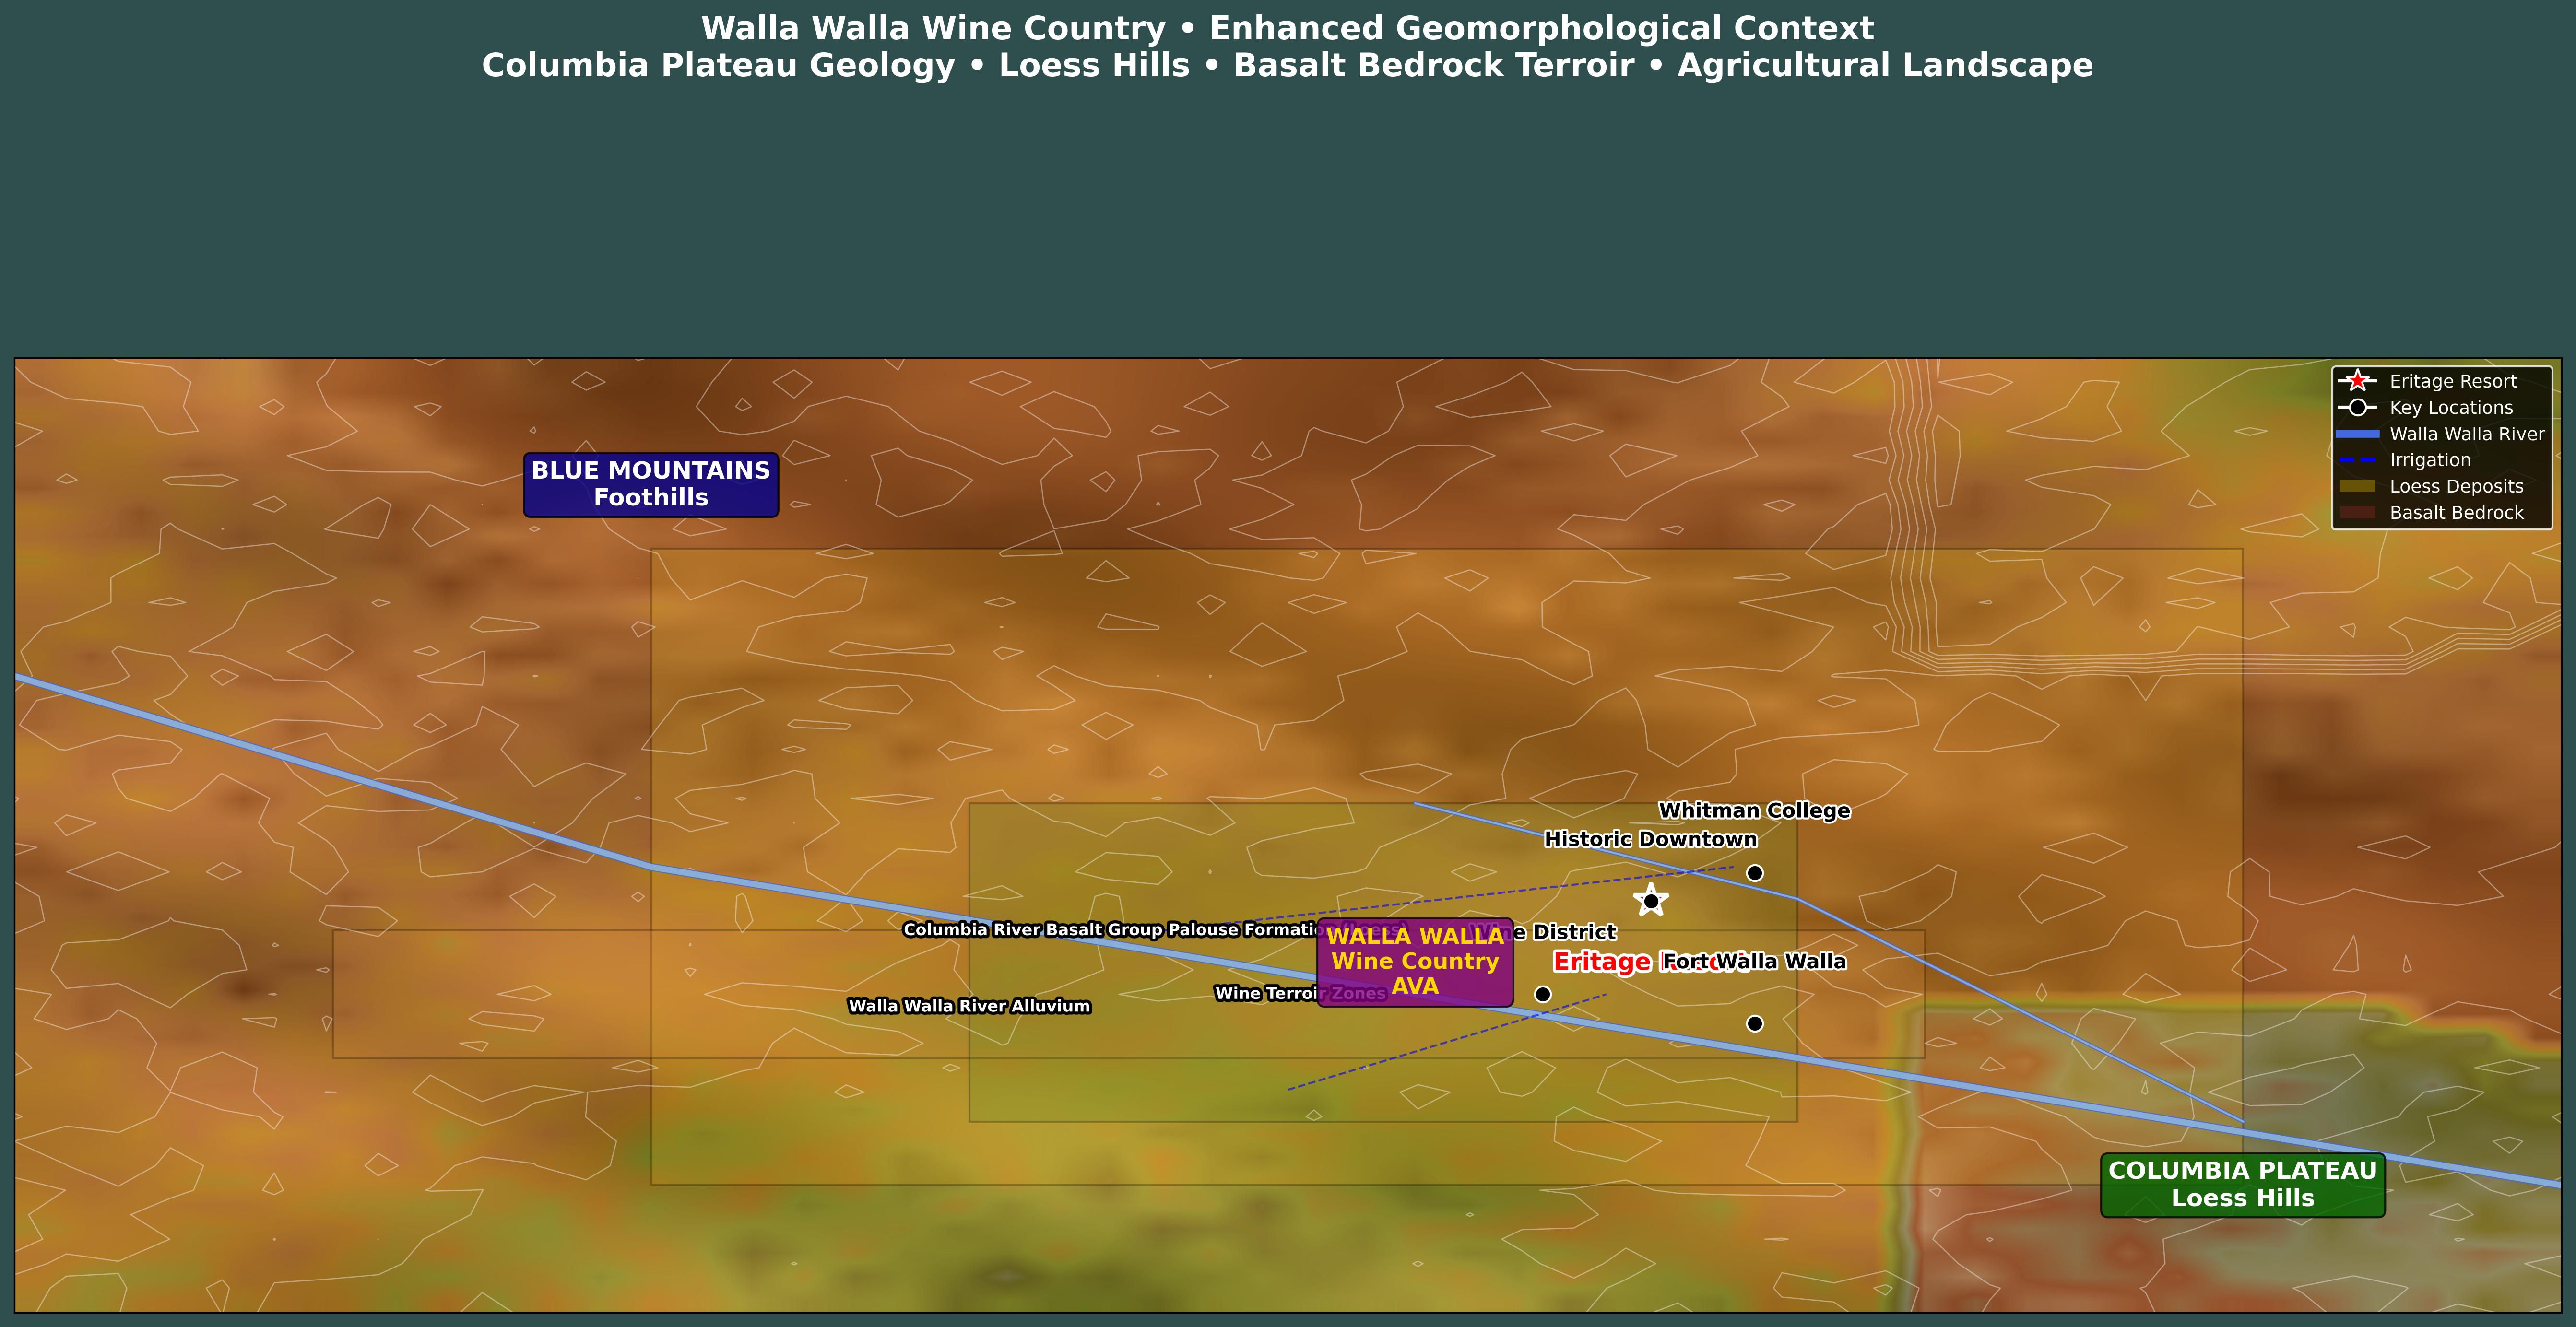
\includegraphics[width=0.9\textwidth]{images/walla_walla_enhanced_geospatial.png}
\caption{\textbf{\textcolor{primary}{WALLA WALLA WINE COUNTRY • Enhanced Geomorphological Context}} \\ 
\textbf{\textcolor{secondary}{Accommodation:}} \textcolor{mapred}{●} Eritage Resort (Red Star) \\
\textbf{\textcolor{secondary}{Geological Features:}} \\
\textcolor{brown}{●} \textcolor{brown}{Columbia River Basalt Group} (15.6 Ma flood basalt foundation) \\
\textcolor{gold}{●} \textcolor{gold}{Palouse Formation Loess} (wind-blown glacial sediment) \\
\textcolor{mapblue}{●} \textcolor{mapblue}{Walla Walla River Valley} (agricultural drainage system) \\
\textcolor{mapgreen}{●} \textcolor{mapgreen}{Wine Terroir Zones} (basalt bedrock with loess soils) \\
\textbf{\textcolor{secondary}{Key Locations:}} \\
\textcolor{mapred}{★} Downtown Historic District • Wine District • Blue Mountains Foothills}
\end{figure}

\begin{center}\rule{0.5\linewidth}{0.5pt}\end{center}

\newpage

\section{\texorpdfstring{\textcolor{primary}{LEG 6: Columbia River Gorge}}{}}\label{section-39}

\subsection{\texorpdfstring{\textcolor{secondary}{August 11, 2025 | 1 Night}}{}}\label{section-40}

\textbf{\textcolor{secondary}{Driving Route:}} Walla Walla → Columbia
River Gorge (205 mi, 3h 37m scenic drive)

\subsubsection{\texorpdfstring{\textcolor{primary}{BOOKING STATUS: ✅ BOOKED!}}{}}\label{section-41}

\textbf{\textcolor{secondary}{Glamping:}} Under Canvas Columbia River\\
\textbf{\textcolor{secondary}{Address:}} 1681 Little White Salmon Rd,
Cook, WA 98605\\
\textbf{\textcolor{secondary}{Website:}} undercanvas.com\\
\textbf{\textcolor{primary}{CONFIRMED:}} King bed with bathroom,
Stargazers tent for August 11, 2025\\
\textbf{\textcolor{primary}{Status:}} ✅ SUCCESSFULLY BOOKED BY SMADAR

\subsubsection{\texorpdfstring{\textcolor{primary}{ROUTE INFORMATION}}{}}\label{section-42}

\textbf{\textcolor{secondary}{From:}} Walla Walla, WA \textbar{}
\textbf{\textcolor{secondary}{Distance:}} 205 miles \textbar{}
\textbf{\textcolor{secondary}{Drive Time:}} 3h 37m\\
\textbf{\textcolor{secondary}{Next Day:}} Drive to Seattle (110 mi, 2h
10m)

\subsubsection{\texorpdfstring{\textcolor{primary}{SPECIAL EXPERIENCES}}{}}\label{section-43}

\begin{itemize}
\tightlist
\item
  \textbf{\textcolor{secondary}{Stargazer Experience}} - Private
  astronomer on clear nights
\item
  \textbf{\textcolor{secondary}{Waterfall tours}} - Multiple Columbia
  River Gorge waterfalls\\
\item
  \textbf{\textcolor{secondary}{Scenic gorge drives}} - Historic
  Columbia River Highway
\end{itemize}

\subsubsection{\texorpdfstring{\textcolor{primary}{DINING \& ACTIVITIES}}{}}\label{section-44}

\begin{itemize}
\tightlist
\item
  \textbf{\textcolor{secondary}{Thunder Island Brewing}} - Local brewery
  with river views
\item
  \textbf{\textcolor{secondary}{Camp dining}} - Under Canvas provides
  campfire cooking\\
\item
  \textbf{\textcolor{secondary}{Morning coffee}} - Served at fire pit
  starting 6 AM
\end{itemize}

\newpage

\section{\texorpdfstring{\textcolor{primary}{LEG 6: Columbia River Gorge Enhanced Geospatial Context}}{}}\label{section-45}

\begin{figure}[H]
\centering
\includegraphics[width=0.9\textwidth]{images/columbia_river_gorge_enhanced_geospatial.png}
\caption{\textbf{\textcolor{primary}{COLUMBIA RIVER GORGE • Enhanced Geomorphological Context}} \\ 
\textbf{\textcolor{secondary}{Accommodation:}} \textcolor{mapred}{●} Under Canvas Columbia River (Red Star) \\
\textbf{\textcolor{secondary}{Geological Features:}} \\
\textcolor{brown}{●} \textcolor{brown}{Columbia River Basalt Group} (Grande Ronde \& Wanapum Basalt) \\
\textcolor{mapblue}{●} \textcolor{mapblue}{Columbia River} (only river through Cascade Range) \\
\textcolor{gray}{●} \textcolor{gray}{Bonneville Landslide} (\~500 years BP natural dam) \\
\textcolor{mapgreen}{●} \textcolor{mapgreen}{Missoula Flood Deposits} (Ice Age megaflood scars) \\
\textcolor{cyan}{●} \textcolor{cyan}{Cascade Range Waterfalls} (erosional alcoves) \\
\textbf{\textcolor{secondary}{Key Locations:}} \\
\textcolor{mapred}{★} Bridge of the Gods • Bonneville Dam • Multnomah Falls • Crown Point}
\end{figure}

\begin{center}\rule{0.5\linewidth}{0.5pt}\end{center}

\newpage

\section{\texorpdfstring{\textcolor{primary}{LEG 7: Seattle, Washington}}{}}\label{section-46}

\subsection{\texorpdfstring{\textcolor{secondary}{August 12, 2025 (Departure Day)}}{}}\label{section-47}

\textbf{\textcolor{secondary}{Driving Route:}} Columbia River Gorge →
Seattle (110 mi, 2h 10m to departure)

\subsubsection{\texorpdfstring{\textcolor{primary}{BOOKING DETAILS}}{}}\label{section-48}

\textbf{\textcolor{secondary}{FLIGHT BOOKING (PRIORITY):}}\\
- \textbf{\textcolor{secondary}{From Seattle (August 12th):}}
Afternoon/evening flight SEA→JFK\\
- \textbf{\textcolor{secondary}{Cost:}} \$249/person \textbar{}
\textbf{\textcolor{secondary}{Flight Time:}} 5h 28m direct Delta\\
- \textbf{\textcolor{secondary}{Book Through:}} Delta.com or travel
agent

\textbf{\textcolor{secondary}{OPTIONAL OVERNIGHT (if late flight):}}\\
\textbf{\textcolor{secondary}{Hotel:}} The Fairmont Olympic Seattle\\
\textbf{\textcolor{secondary}{Address:}} 411 University St, Seattle, WA
98101\\
\textbf{\textcolor{secondary}{Phone:}} (206) 621-1700 \textbar{}
\textbf{\textcolor{secondary}{Rate:}} \$400-600/night

\subsubsection{\texorpdfstring{\textcolor{primary}{ROUTE INFORMATION}}{}}\label{section-49}

\textbf{\textcolor{secondary}{From:}} Columbia River Gorge \textbar{}
\textbf{\textcolor{secondary}{Distance:}} 110 miles \textbar{}
\textbf{\textcolor{secondary}{Drive Time:}} 2h 10m

\subsubsection{\texorpdfstring{\textcolor{primary}{PRE-DEPARTURE ACTIVITIES}}{}}\label{section-50}

\begin{itemize}
\tightlist
\item
  \textbf{\textcolor{secondary}{Pike Place Market}} - Morning visit
  before flight
\item
  \textbf{\textcolor{secondary}{Seattle waterfront}} - Final Pacific
  Northwest views\\
\item
  \textbf{\textcolor{secondary}{Coffee culture}} - Starbucks Reserve or
  local roasters
\end{itemize}

\subsubsection{\texorpdfstring{\textcolor{primary}{AIRPORT LOGISTICS}}{}}\label{section-51}

\begin{itemize}
\tightlist
\item
  \textbf{\textcolor{secondary}{Car Return}} - Allow 2+ hours before
  flight
\item
  \textbf{\textcolor{secondary}{Seattle-Tacoma International (SEA)}} -
  Large airport, arrive early
\end{itemize}

\newpage

\section{\texorpdfstring{\textcolor{primary}{LEG 7: Seattle Enhanced Geospatial Context}}{}}\label{section-52}

\begin{figure}[H]
\centering
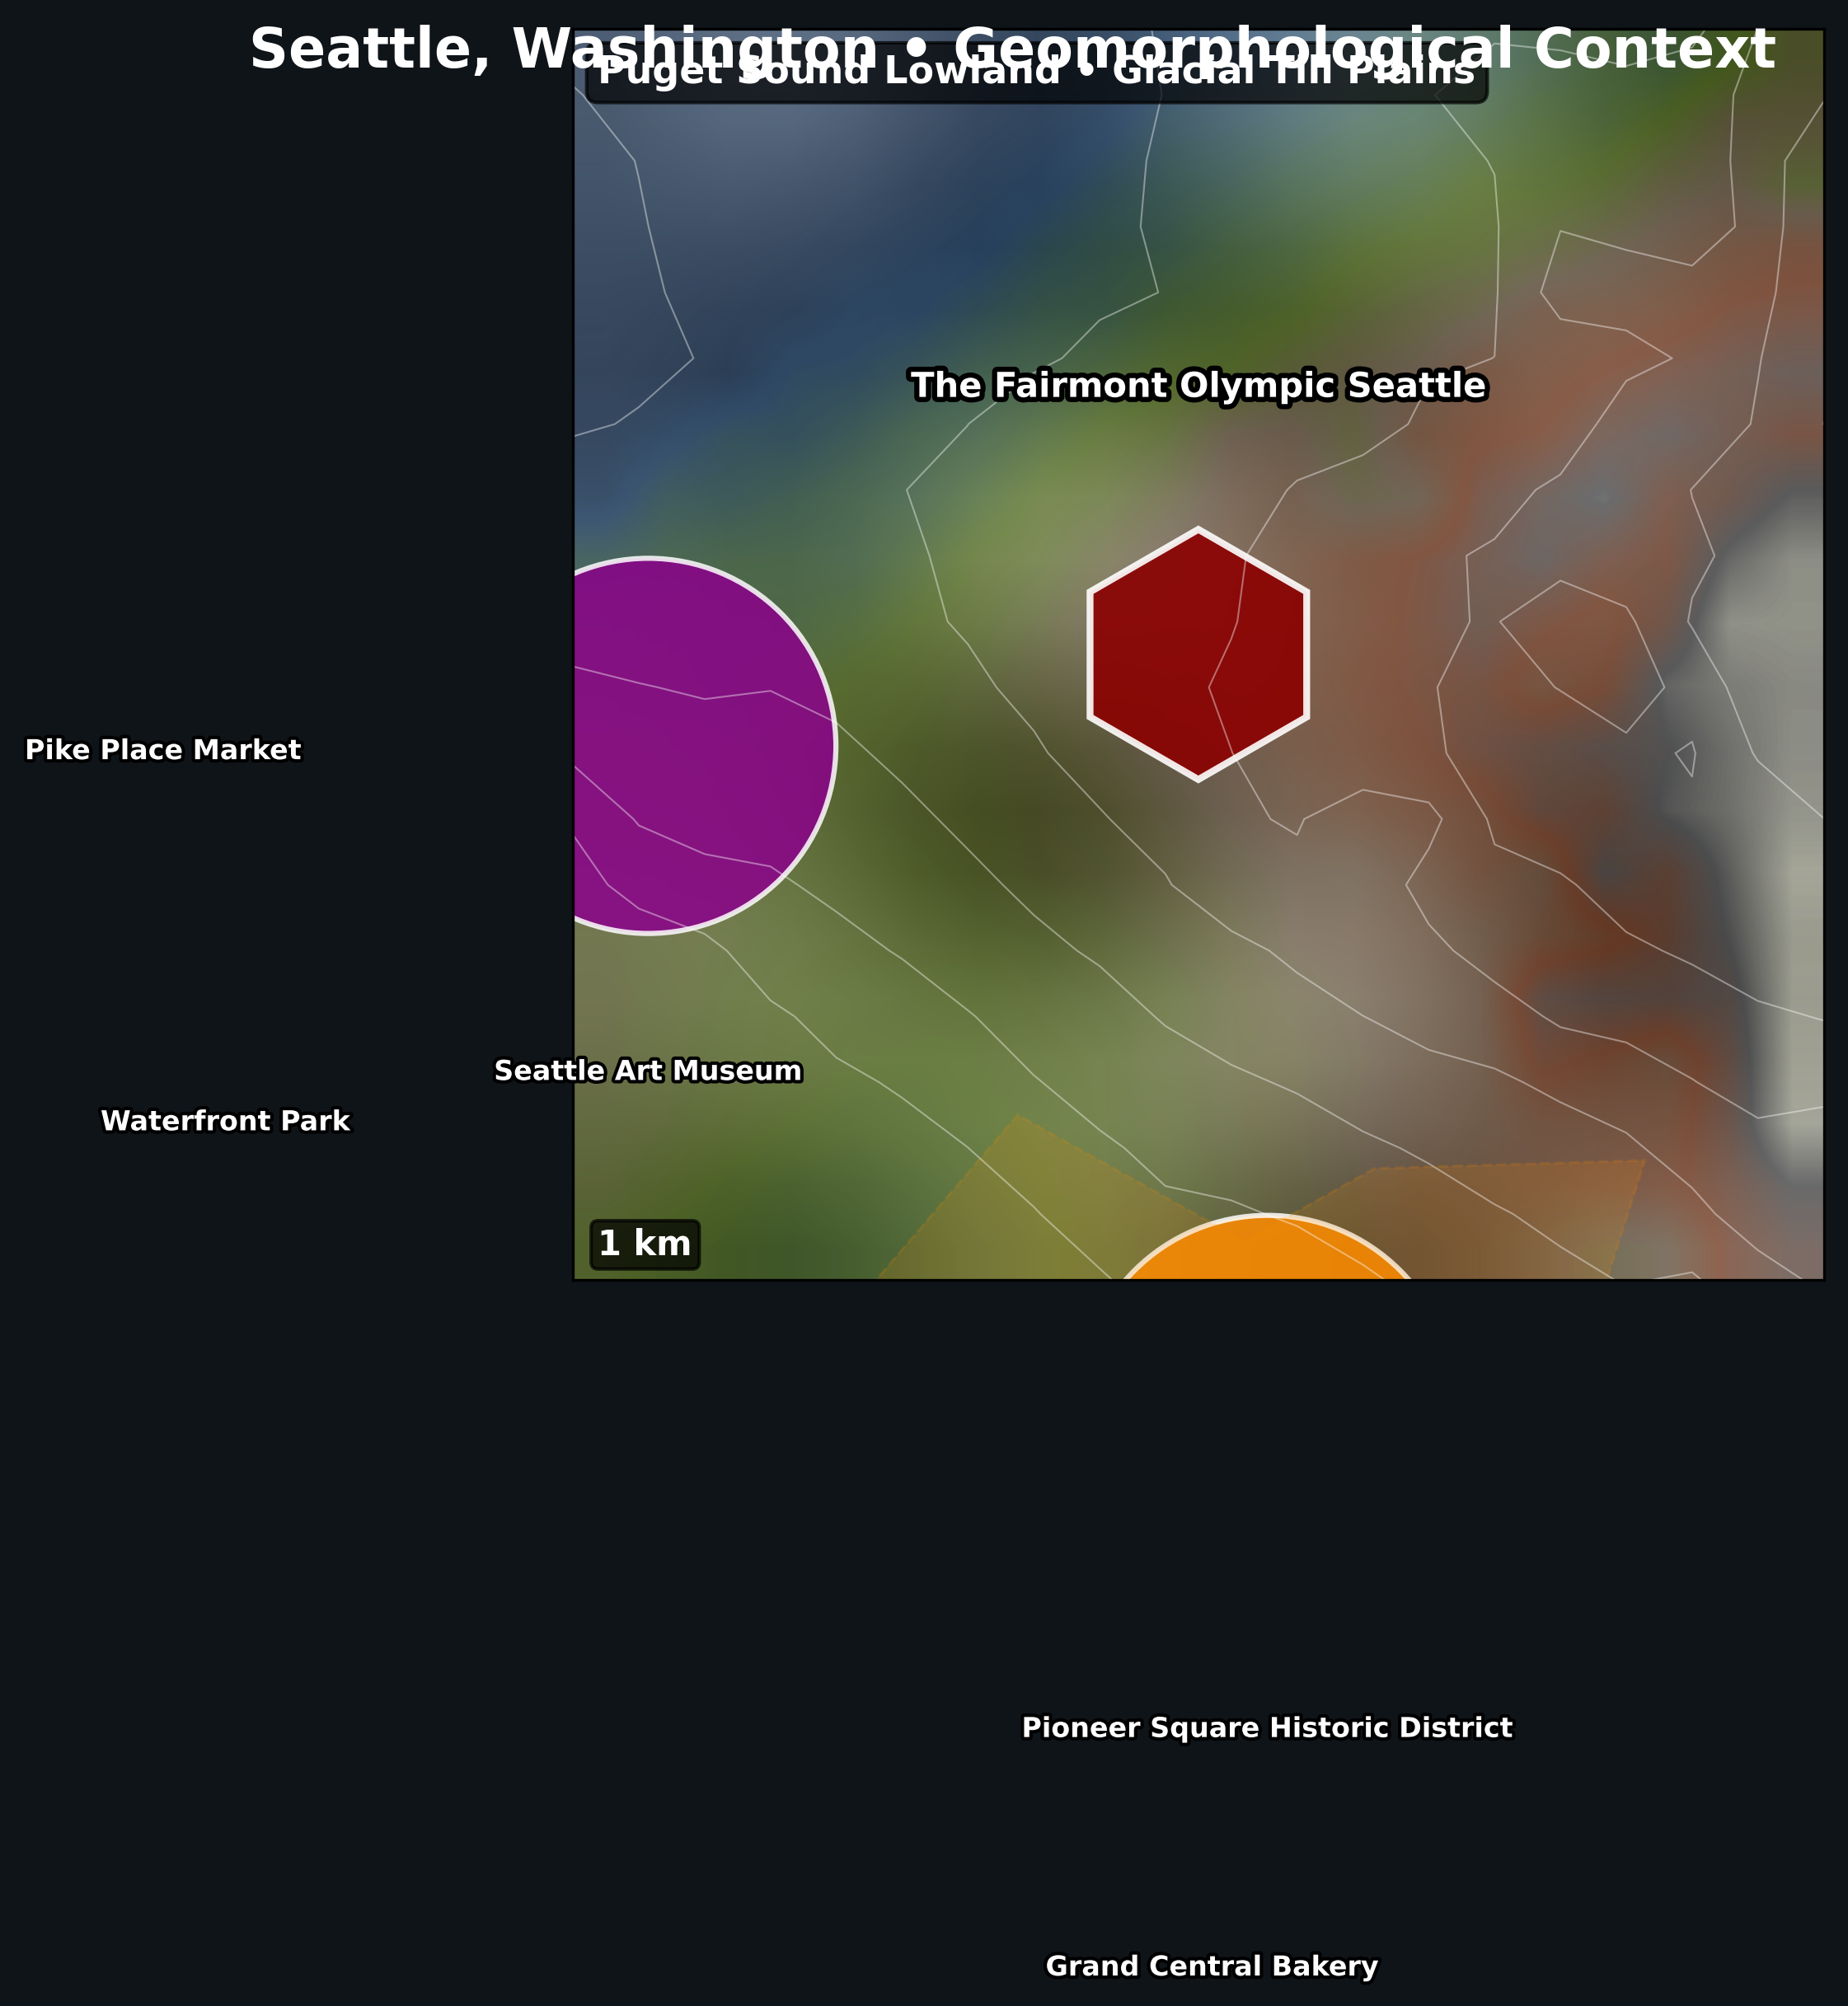
\includegraphics[width=0.9\textwidth]{images/seattle_wa_geomorphological_map.png}
\caption{\textbf{\textcolor{primary}{SEATTLE \& PUGET SOUND • Enhanced Geomorphological Context}} \\ 
\textbf{\textcolor{secondary}{Accommodation:}} \textcolor{mapred}{●} The Fairmont Olympic Seattle (Red Star) \\
\textbf{\textcolor{secondary}{Geological Features:}} \\
\textcolor{brown}{●} \textcolor{brown}{Puget Sound Lowland} (glacial trough) \\
\textcolor{mapblue}{●} \textcolor{mapblue}{Elliott Bay} (glacial carved embayment) \\
\textcolor{gray}{●} \textcolor{gray}{Vashon Till} (glacial sediment deposits) \\
\textcolor{mapgreen}{●} \textcolor{mapgreen}{Cascade Range} (volcanic arc backdrop) \\
\textbf{\textcolor{secondary}{Key Locations:}} \\
\textcolor{mapred}{★} Pike Place Market • Seattle Waterfront • Pioneer Square • Seattle Center}
\end{figure}

\begin{center}\rule{0.5\linewidth}{0.5pt}\end{center}

\newpage

\section{\texorpdfstring{\textcolor{primary}{Quick Reference: All Booking Contacts}}{}}\label{section-53}

\subsection{\texorpdfstring{\textcolor{secondary}{COMPLETED BOOKINGS ✅}}{}}\label{section-54}

\begin{itemize}
\tightlist
\item
  \textbf{\textcolor{primary}{Kimpton Armory Hotel Bozeman}} (Aug 3-5) -
  Two King Rooms
\item
  \textbf{\textcolor{primary}{Under Canvas Columbia River Gorge}} (Aug
  11) - Stargazers Tent
\end{itemize}

\subsection{\texorpdfstring{\textcolor{secondary}{REMAINING TO BOOK}}{}}\label{section-55}

\begin{table}[H]
\centering
\begin{tabular}{|l|l|l|l|}
\hline
\textbf{Location} & \textbf{Hotel} & \textbf{Phone} & \textbf{Rate/Night} \\
\hline
\textcolor{primary}{Missoula} & AC Hotel Downtown & (406) 541-8000 & \$455 \\
\hline
\textcolor{primary}{McCall} & LA CASA ITALIANA Condo & Vacation rental platform & \$360/night \\
\hline
\textcolor{primary}{Joseph} & Little Brick Building + Room \#11 & Book direct & \$667/night (both) \\
\hline
\textcolor{primary}{Walla Walla} & Eritage Resort & Contact needed & \$400-600 \\
\hline
\textcolor{primary}{Seattle} & Fairmont Olympic & (206) 621-1700 & \$400-600 \\
\hline
\end{tabular}
\end{table}

\subsection{\texorpdfstring{\textcolor{secondary}{ESTIMATED TOTAL COSTS}}{}}\label{section-56}

\textbf{\textcolor{primary}{Flights:}} \$716 per couple (\$109 + \$249 ×
2)\\
\textbf{\textcolor{primary}{Hotels:}} \$2,890 for 8 nights total\\
\textbf{\textcolor{primary}{Meals/Activities:}} \$1,000-1,500\\
\textbf{\textcolor{primary}{TOTAL ESTIMATE:}} \$4,606-5,106 per couple

\subsection{\texorpdfstring{\textcolor{secondary}{BOOKING STRATEGY}}{}}\label{section-57}

\begin{enumerate}
\def\labelenumi{\arabic{enumi}.}
\tightlist
\item
  \textbf{\textcolor{primary}{Book flights IMMEDIATELY}} (save \$280+
  per couple) - HIGHEST PRIORITY
\item
  \textbf{\textcolor{primary}{LA CASA ITALIANA McCall}} (Aug 6-8) - Book
  the downtown condo\\
\item
  \textbf{\textcolor{primary}{The Jennings Hotel Joseph}} (Aug 8-9) -
  Both rooms\\
\item
  \textbf{\textcolor{primary}{Remaining accommodations}} - Missoula,
  Walla Walla, Seattle\\
\item
  \textbf{\textcolor{primary}{Consider travel insurance}} for peace of
  mind
\end{enumerate}

\begin{center}\rule{0.5\linewidth}{0.5pt}\end{center}

\textbf{\textcolor{primary}{Created for Smadar's Pacific Northwest Adventure}}\\
\textbf{\textcolor{secondary}{Safe travels and amazing experiences ahead!}}




\end{document}
